% Note that if you want something in single space you can go back and
% forth between single space and normal space by the use of \ssp and
% \nsp.  If you want doublespacing you can use \dsp.  \nsp is normally
% 1.5 spacing unless you use the doublespace option (or savepaper
% option)
%
%(FORMAT) Usually you *don't* want to mess with the spacing for your
%(FORMAT) final version.  If you think/know that the thesis template
%(FORMAT) and/or thesis style file is incorrect/incomplete, PLEASE
%(FORMAT) contact the maintainer.  THANK YOU!!!

\chapter{BINARY SEARCH TREES}
\label{chap:binarysearchtree}
% By labeling the chapter, I can refer to it later using the
% label. (\ref{chap:binarysearchtree}, \pageref{chap:binarysearchtree}) Latex will take care
% of the numbering.

The single most heavily used data structure in line sweep algorithm is binary search tree (BST), hence it is worth to spend an entirely dedicated chapter to explain this data structure and how it is used in this algorithm. Although the algorithm uses slightly modified binary search tree but still the main concept is that of a binary search tree. In fact the algorithm uses an AVL tree. Hence it is imperative to understand this data structure in order to properly understand the working of the algorithm.

\section{Definition and Properties}

In computer science, a binary search tree (BST), which may sometimes also be called an ordered or sorted binary tree, is a node-based binary tree data structure which has the following properties \cite{BSTWIKI}:
\begin{itemize}
	\item The left subtree of a node contains only nodes with keys less than or equal to the node's key.
	\item The right subtree of a node contains only nodes with keys greater than the node's key.
	\item Both the left and right subtrees must also be binary search trees.
\end{itemize}

Since each node in a binary search tree has only two child nodes and hence the name binary search tree. The only exception to the nodes having two child nodes is the bottom node where it does not have any child node. These nodes are sometimes also referred to as a leaf node.

\section{Terms}

Each node in a binary search tree stores some useful data. This data can be as simple as storing an integer value or as complex as storing an object of a very complex class which can contain thousands of lines of code. The data that is stored in each node depends on the applications context in which the binary search tree is going to be used and the requirement of the application. Binary search tree is the fundamental data structure used to construct more complex data structures such as link-list, queue, sets, multisets and associative arrays. 

The number of levels of a binary search tree is called as its height. The height normally does not include the node itself. Thus the height of a binary tree is essentially the depth of the tree. A balanced binary tree is a tree where the heights of the left and right subtrees are equal. The size of a binary tree is the total number of nodes in the tree. These nodes include the root node, leaf nodes and any intermediate child nodes. An empty tree has size of zero (0). Figure.~\ref{fig14} represents a binary search tree of size 9 and depth 3, with root 20 and leaves 7, 11, 16 and 27. The tree is not balanced.
\begin{figure}[ht]
  \begin{center}
   	\fbox{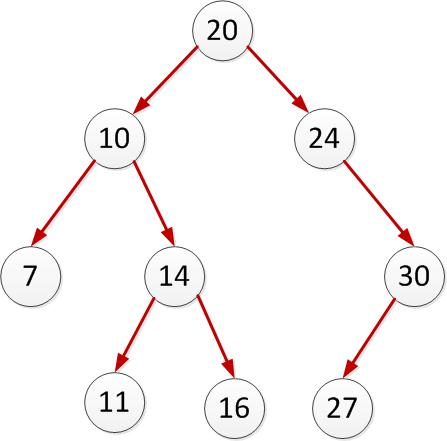
\includegraphics[width=3in, height=3in]{Figures/Figure14}}
  \end{center}
  \centering
	\parbox{3in}{\caption{A binary tree.} \label{fig14}} 
\end{figure}

\section{AVL Tree}

The Line Sweep Algorithm uses an AVL tree instead of a binary tree. The AVL tree is named after its two Soviet inventors, G. M. Adelson-Velskii and E. M. Landis, who published it in their 1962 paper ``An algorithm for the organization of information". \cite{AVL} An AVL tree is pretty much similar to a binary search tree except for the fact that it is a self-balancing binary search tree. The AVL tree is named after its two inventors, G.M. Adelson-Velskii and E.M. Landis. In an AVL tree the heights of two child subtrees of any node differ by at most one. The insertion or deletion operations on an AVL tree may require the tree to be rebalanced by one or more tree rotations.

The balance factor of each node is the height of its left subtree minus the right subtree. Sometimes this can be opposite but in our implementation it is the height of the left subtree minus the right subtree. This height is stored in each node and kept updated at any particular instance of time. A node with a balance factor of 1, 0 or -1 is considered as balanced. In other words we perform rotation operations whenever the balance factor of any node becomes either 2 or -2. In these situations we perform the rotation operations in order to balance the AVL tree.

\section{Special Algorithm Requirement}

In our implementation, according to the text book \cite{TEXTBOOK1} we store some special data in each internal node. Each internal node stores the right-most child in its left subtree. Theoretically each internal node should store some data that guides the path to the destination node where the actual data is stored. So instead of storing the segments in internal nodes we store the right most segment in its left subtree. While finding a particular segment we test if the segment lies to the left or right of the segment stored in the internal node and descend accordingly based on the outcome. Eventually we would reach the leaf node. Each Update and Delete operation takes {\it O}(log n) time.

\section{Tree Rotations}

Tree rotations are done mainly in order to balance the tree. There are primarily two kinds of tree rotations namely left rotation and right rotation. These rotations are pictorially represented in the Figure.~\ref{fig15}.
\begin{figure}[ht]
  \begin{center}
   	\fbox{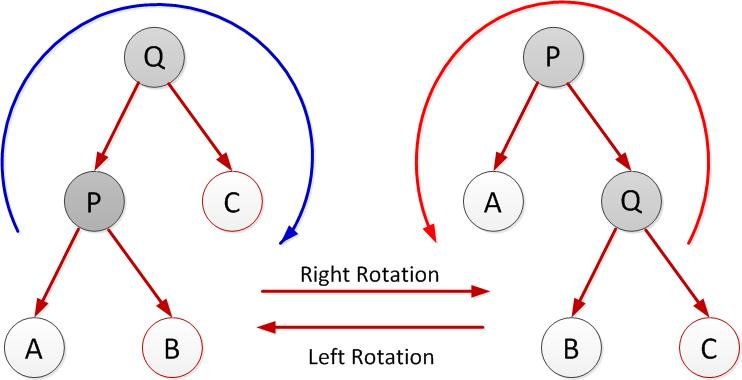
\includegraphics[width=5in, height=2.5in]{Figures/Figure15}}
  \end{center}
  \centering
	\parbox{5in}{\caption{Left and right rotations of a tree.} \label{fig15}} 
\end{figure}

The right rotation operation is performed in Figure ~\ref{fig15} with Q as the root. This operation results in a tree structure as shown on the right side by performing rotation in clockwise direction of the tree shown on the left side. Similarly the left rotation is performed in the inverse direction rooted at node P. This results in a tree structure as shown in the left side by performing rotation on anticlockwise direction of the tree shown on right side. There are a few rules that must be followed while performing rotations. These rules are -
\begin{enumerate}
	\item The order of the leaves prior to rotation and post rotation must remain the same. In other words the order of the leaves in the depth first search should remain the same before and after the rotation.
	\item For any particular node the right child must always be greater than or equal to the parent node and the left child must be less than the parent node. This is the basic property of a binary search tree which needs to be followed by tree rotations.
\end{enumerate}

It thus implies that the leaf nodes can change the parent nodes after rotation but they still follow the two rules stated above. Both the left and right rotations should preserve the integrity of the tree which balancing the tree.

\section{Importance of balacing a tree}

If we do not balance the tree then either the left or right subtree will continue to increase at an exponential rate than the other corresponding subtree. This can significantly affect the performance for lookup and would become linear in the worst case scenario. If only the left or right subtree continue to grow then the data structure would no longer be a tree but would be a linked list.

\section{Tree rotations in order to balance a tree}

As we stated before a tree rotation is performed as soon as the balance factor of any node becomes either 2 or -2. If we interpret the meaning of the balance factor of 2 or -2 then it can be easily understood that either the left or the right subtree is 2 nodes greater in height than the other corresponding subtree. If this were not the case then the balance factor would never be 2 or -2. When a subtree is rotated, the subtree side upon which it is rotated decreases its height by one while the other subtree increases its height by one. This makes tree rotations as a useful tool in rebalancing the tree. There are four conditions that can cause the rotation of tree to be triggered.  In some scenarios only a single rotation will not rebalance the tree. Consider the left right and the right left case as given in Figure.~\ref{fig16} \cite{TREEROTWIKI}. In the case of the left right case initially a left rotation is performed on the right child of the left child of node whose balance factor triggered the rotation so that the tree structure becomes like a left left case. Then again a right rotation is performed on the node that triggered the rotation. Similarly corresponding opposite steps is performed for a right left case. Note that these extra steps are taken so that the rotations follow the two rules stated previously in this chapter in order to maintain the integrity of the tree. The steps can be summarized by a small table, given by Table \ref{tab1}.
\begin{figure}[ht]
  \begin{center}
   	\fbox{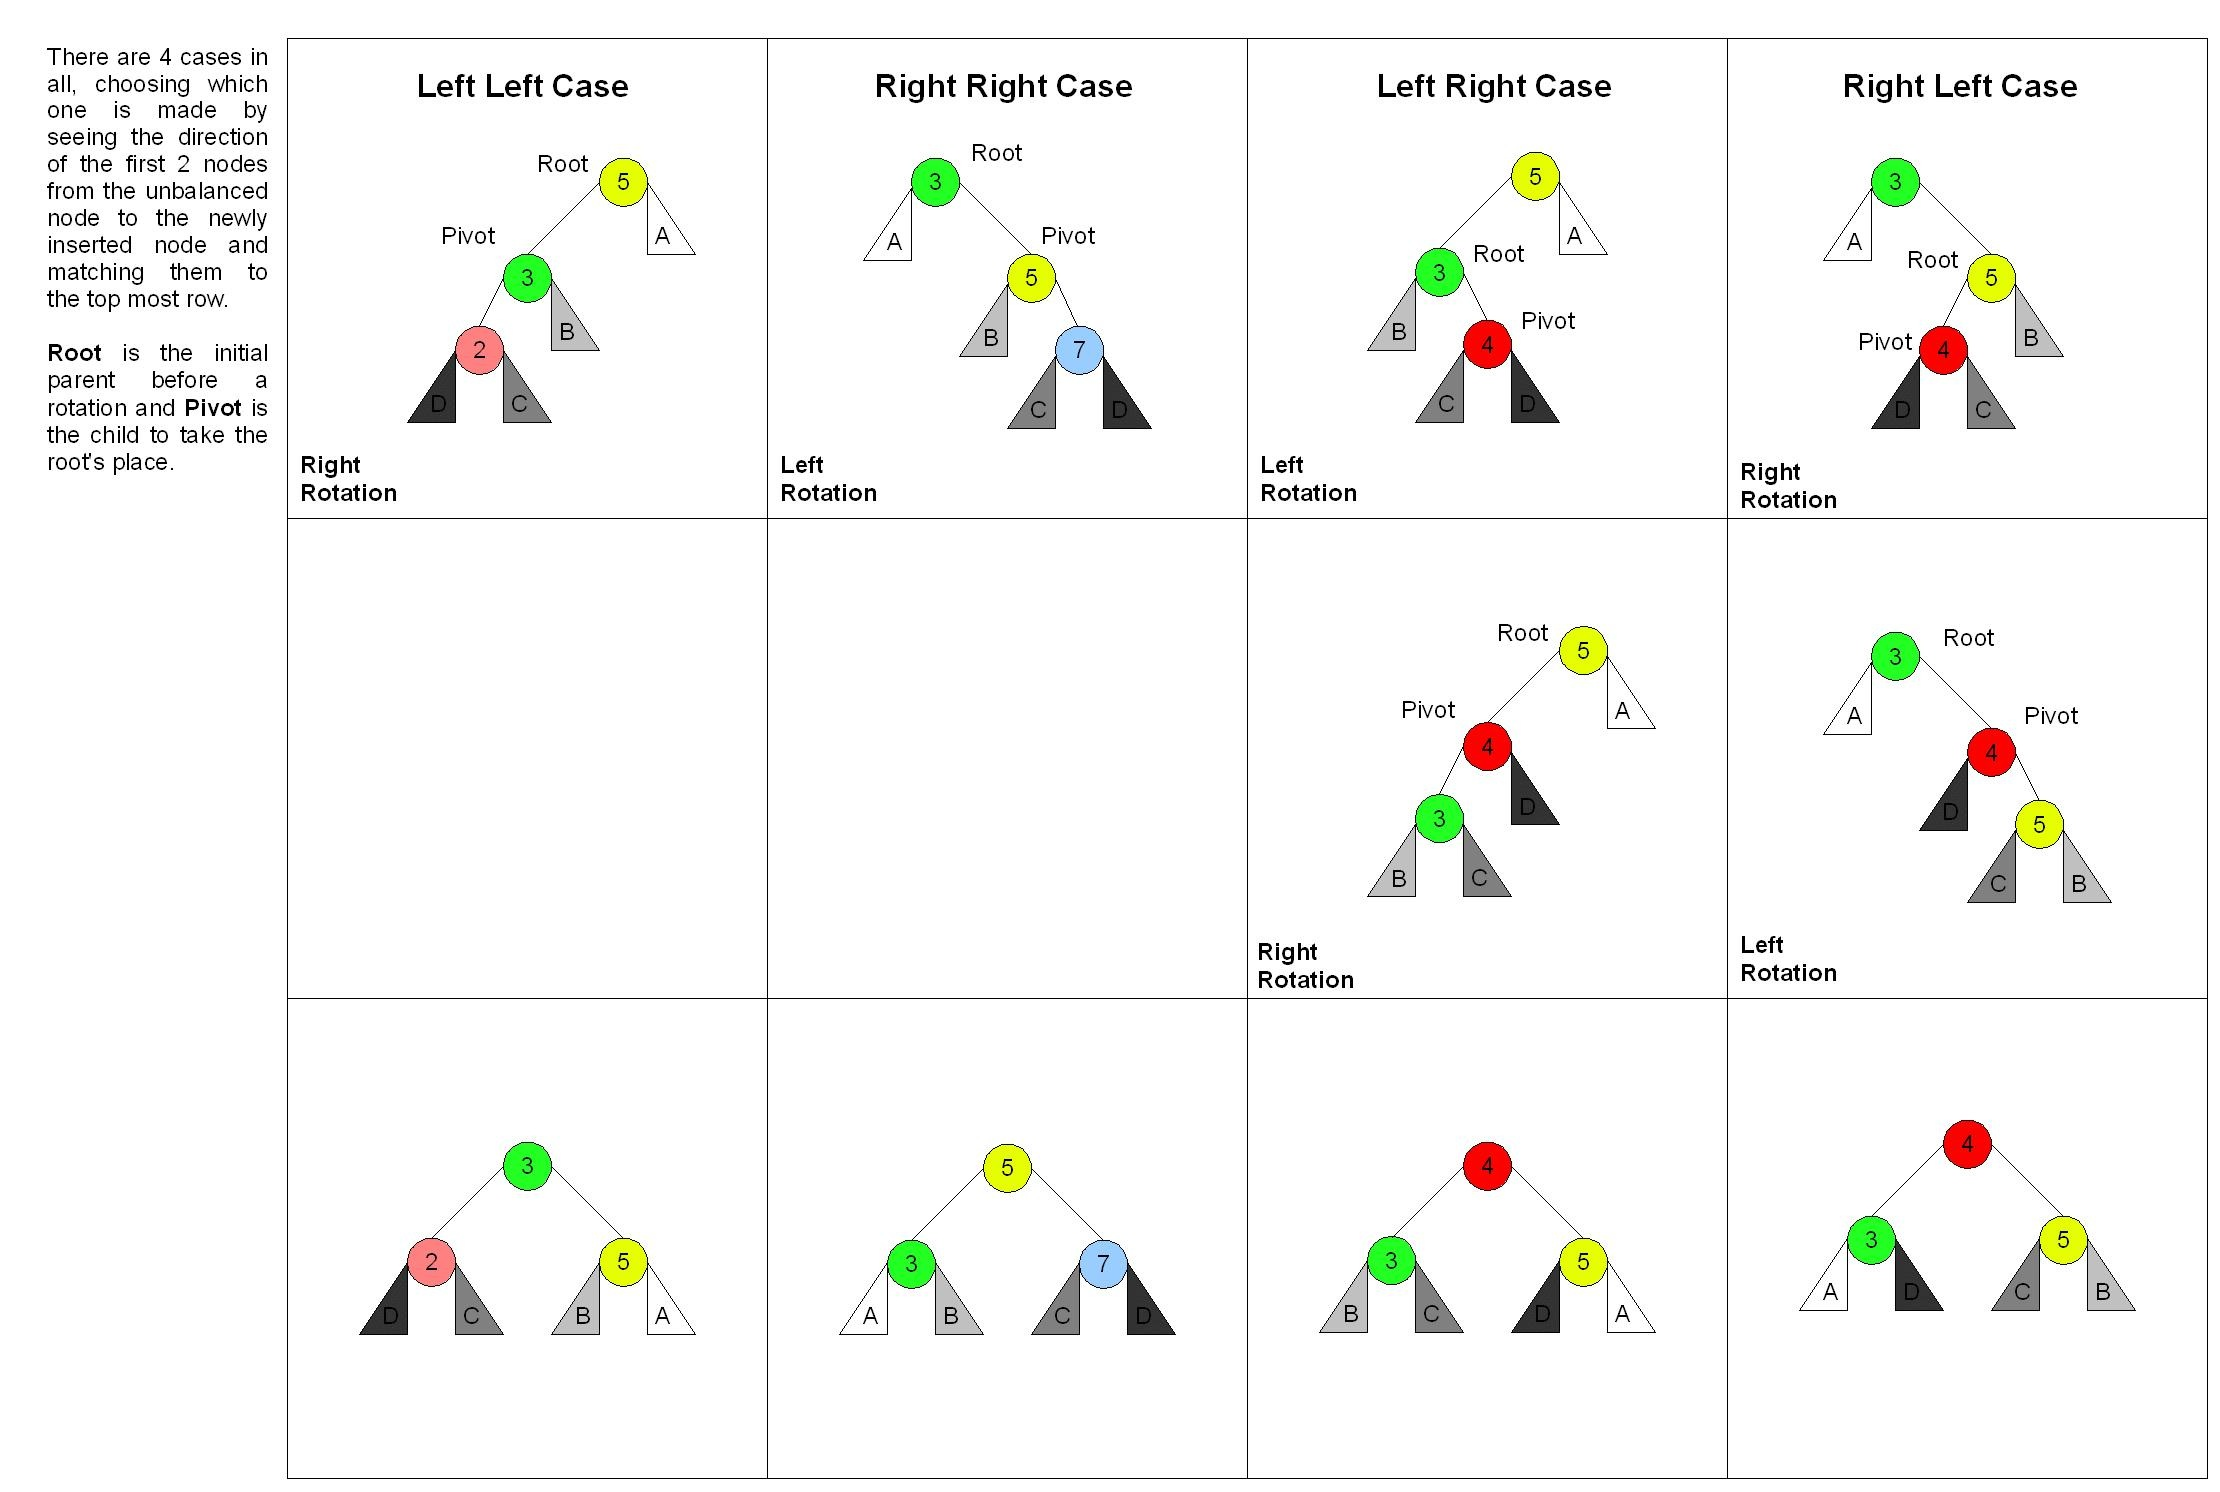
\includegraphics[width=6.5in, height=7in]{Figures/Figure16}}
  \end{center}
  \centering
	\parbox{6.5in}{\caption{Pictorial representation of rotations causing rebalancing in an AVL tree. Source: WIKIPEDIA, \textbf{\textit{Tree balancing - Wikipedia, the free encyclopedia}}. Tree Rebalancing, http://en.wikipedia.org/wiki/File:Tree Rebalancing.gif, accessed Aug. 2012, n.d.} \label{fig16}} 
\end{figure}

\clearpage
\begin{table}[hbt]
\centering
  \begin{minipage}{5in}
    \caption{Steps Required to Balance Tree After Node Insertion\label{tab1}}
    \begin{tabular}{||p{2.5cm}|p{2.5cm}|p{2.5cm}|p{4.5cm}||}    \hline
      Node Balance Factor &	Left Subtree Balance Factor  &  Right Subtree Balance Factor & Steps \\ \hline \hline
      -2 & - & -1  & Perform Left Rotation \\ \hline
	  -2 & - & 1  & Perform Right Rotation and Perform Left Rotation \\ \hline
	   2 & 1 & -  & Perform Right Rotation \\ \hline
       2 & -1 & -  & Perform Left Rotation and Perform Right Rotation \\ \hline
    \end{tabular}
  \end{minipage}
\end{table}

The rotation operations, given in Table \ref{tab1} are triggered whenever a particular node is deleted. Besides these operations there is one more additional step that needs to be performed which is specific only when a node is deleted from a tree, given by Table \ref{tab2}. These operations are specifically executed whenever a particular node is deleted from an AVL tree. (Note that these are the additional operations, which needs to be performed along with the operations given in Table \ref{tab1}).
\begin{table}[hbt]
\centering
  \begin{minipage}{5in}
    \caption{Extra Steps Required to Balance Tree After Node Deletion\label{tab2}}
    \begin{tabular}{||p{2.5cm}|p{2.5cm}|p{2.5cm}|p{4.5cm}||}    \hline
      Node Balance Factor &	Left Subtree Balance Factor  &  Right Subtree Balance Factor & Steps \\ \hline \hline
      -2 & 0 & -  & Perform Right Rotation \\ \hline
	   2 & - & 0  & Perform Left Rotation and Perform Left Rotation \\ \hline
	\end{tabular}
  \end{minipage}
\end{table}

The concepts, rules and operations mentioned until now are the general AVL tree rule�s that needs to be followed by any implementation of an AVL tree. The advanced line sweep algorithm also has one more additional rule that needs to be followed. Each internal node needs to store the right most child node in the left subtree. This rule is extremely challenging to be followed because this is the only thing that is mentioned about the rule in the text book [1]. There is no implementation details stated as to how this rule should be followed. This is also challenging because the internal nodes also needs to be adjusted whenever a particular node is inserted or deleted from the AVL tree. The implementation needs to make sure that the tree rotation does not violate this rule. Thus one more rule has been added besides the two previous rules for tree rotation. We manage to maintain the integrity of the whole tree along with the internal node rules. This is not a trivial task and it took me almost a month to come up with the solution. I have narrowed down the task by breaking it into finite number of steps so that it can be easy to program.

\section{Tree Node Insertion}
\begin{enumerate}
	\item No special thing as such needs to be done when inserting the root node.
	\item If the new node is being inserted as the left node of an already existing node (parent node) and there is no right child for the parent node (Figure.~\ref{fig17}) then insert a new node as the parents right child with the data same as the parent node and copy the data of the left child to the parent node. For instance in Figure ~\ref{fig17}, a new node 2 was inserted to the left of node 4 since 2 is less than 4. Then we created a new node with the same data as the root node as inserted it to the right of the parent node. Also we changed the data of the root node to be the same as the left node�s data.
	\item There would never be a situation where the new node is being inserted as the left node of an already existing node (parent node) and there is an existing right child of the parent node.
	\item Similarly there would never be a situation where the new node is being inserted as the right node of an already existing node (parent node) and there is an existing left child of the parent node.
	\item Rules 3 and 4 hold true because we will always insert/ delete a leaf node and adjust the other corresponding node during insertion/ deletion.
	\item If the new node is being inserted as the right node of an already existing node (parent node) and there is no left child of the parent node (Figure.~\ref{fig18}) then simply insert the new node as the right child of the parent node and insert a new left child of the parent node having the same data as the parent node. Also we need to copy the data of the right child of the parent to the parent of its left most parent. This step will make sure that the internal node is also adjusted properly.
\end{enumerate}
\begin{figure}[ht]
  \begin{center}
   	\fbox{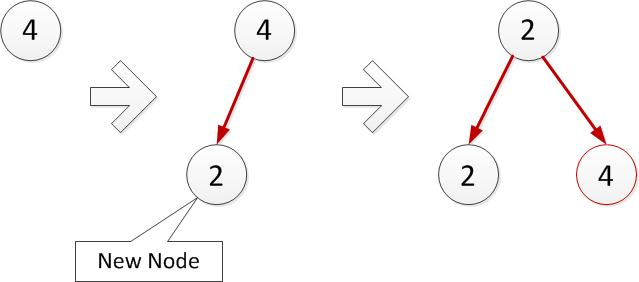
\includegraphics[width=5in, height=2in]{Figures/Figure17}}
  \end{center}
  \centering
	\parbox{5in}{\caption{Inserting a new left leaf node.} \label{fig17}} 
\end{figure}
\begin{figure}[ht]
  \begin{center}
   	\fbox{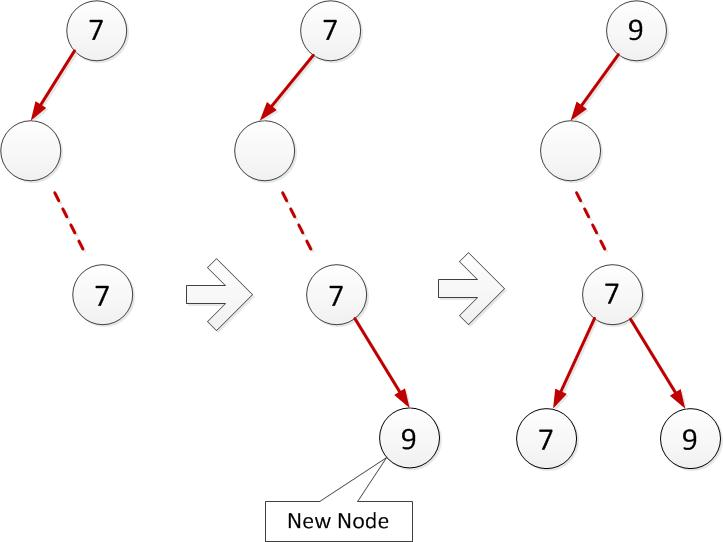
\includegraphics[width=5in, height=3in]{Figures/Figure18}}
  \end{center}
  \centering
	\parbox{5in}{\caption{Inserting a new right leaf node.} \label{fig18}} 
\end{figure} 
\section{Tree Node Deletion}
\begin{enumerate}
	\item If we are deleting the root node explicitly (not in order to maintain the internal nodes) then it should be the only node in the tree. In other words when we are deleting the root node explicitly then it should not have any children.
	\item If the node that we are deleting is a left child and its parent is a root node (Figure.~\ref{fig19}) then it implies that the root node�s data and its left child (the node to be deleted) are the same. Hence we delete both the root node and its left child and make the root node�s right child as the new root node.
	\item If the node that we are deleting is a left child of some parent node (Figure.~\ref{fig20}) and that parent node is not a root node then we delete both the parent node and its left child (the node that we wanted to delete originally) and set the parent�s right child as the child of the parents parent node. This right child would be a right child if the parent node was also a right child of its parent otherwise it would be a left child.
	\item If the node that we are deleting is a right child of some parent (Figure.~\ref{fig21}), then we get its left most parent node. The parent node of its left most parent node must be equal to the node that we want to delete. Hence we delete the parent of the left most parent node and the node that we want to delete and adjust pointers accordingly.
	\item Each time we make adjustment, we need to make sure that the root node is updated correctly if needed and that the AVL tree follows the basic 3 rules stated earlier in this chapter.
\begin{figure}[ht]
  \begin{center}
   	\fbox{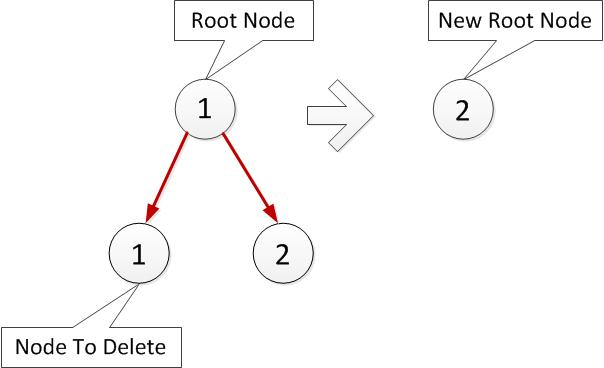
\includegraphics[width=4.5in, height=2.5in]{Figures/Figure19}}
  \end{center}
  \centering
	\parbox{4.5in}{\caption{Deleting left child of root node of height one.} \label{fig19}} 
\end{figure}
\begin{figure}[ht]
  \begin{center}
   	\fbox{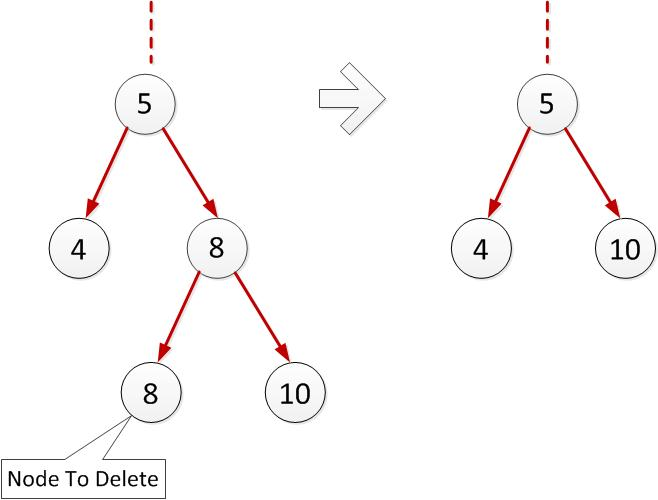
\includegraphics[width=4in, height=2.30in]{Figures/Figure20}}
  \end{center}
  \centering
	\parbox{4in}{\caption{Deleting a left leaf.} \label{fig20}} 
\end{figure}
\end{enumerate}
\begin{figure}[ht]
  \begin{center}
   	\fbox{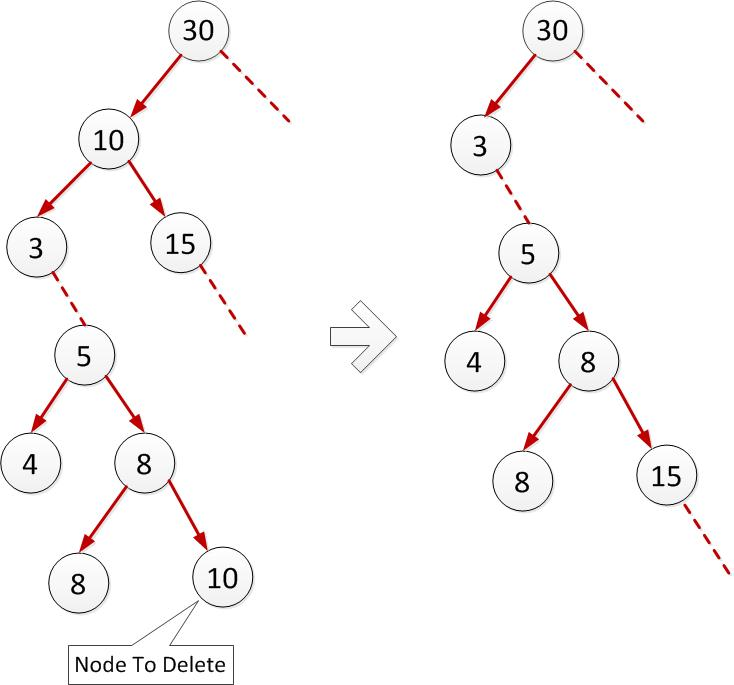
\includegraphics[width=4in, height=4.5in]{Figures/Figure21}}
  \end{center}
  \centering
	\parbox{4in}{\caption{Deleting a right leaf.} \label{fig21}} 
\end{figure}

It is a very important point to be worth noted that each time a node is inserted or deleted then the balance factor must be calculated for all the nodes starting from the inserted node or the parent of the deleted node up to the root node and rotations be performed if needed in order to balance the tree.